\documentclass[a4paper, 11pt]{article}

\usepackage[a4paper, total={6.5in, 8.5in}]{geometry}
\usepackage[round]{natbib}

\usepackage[hyphens]{url}
\usepackage[hidelinks]{hyperref}

\usepackage[parfill]{parskip}
\usepackage{dirtytalk}

\usepackage{graphicx}
\usepackage{multicol}

%opening
\title{Semantic Web Technology -- Assignment 1}
\author{Leon F.A. Wetzel\\s3284174\\ \texttt{l.f.a.wetzel@student.rug.nl}}

\begin{document}

\maketitle

\section{Introduction}

In this report, we take a closer look at two systems designed for the task of named entity linking. We use different English corpora to evaluate the performance of both systems and to determine if they perform well or not. Altough there are a number of systems capable of named entity linking, we only take a look at \textbf{TextRazor} and \textbf{OpenTapioca} as this fits in the scope of the actual assignment. As describing both models does not fall in the scope of this assignment, we refer to the documentation of TextRazor \citep{crayston_2020} and OpenTapioca \citep{DBLP:journals/corr/abs-1904-09131} for more information about their respective history and architecture.

This report covers several aspects of these systems. We take a look at the data which we will use for the evaluation, we discover more about the metrics used for the evaluation and we take an in-depth look at the actual annotations that were generated by these systems.

\section{Data}

Our test data for evaluating the entity linking systems is fairly simple. We use two English news articles which will be annotated by both systems independently. The first news article is a sample from \citet{mcgee_2020}, which covers the situation in Britain regarding new, controversial legislation for Brexit. The second news article is a sample from \citet{mckeever_2020} and explains more about upcoming COVID-19 vaccins. Both articles have been picked based on presence of named entities and differing topic.

Let's take a look at the corpora. Our sample from \citet{mcgee_2020} contains the following text:

\say{
	Ahead of a very crucial round of talks between London and Brussels over the future trading relationship between the UK and the European Union, the British government made a startling admission: That it would be prepared to break the terms of an international treaty.
	The threat was relatively technical -- over an aspect of the withdrawal agreement that allowed the UK to leave the EU at the end of January -- but the admission by a government minister in the House of Commons sent shockwaves through diplomatic circles and raised questions about whether the UK can be trusted on the world stage.
}

We can already spot several named entities by hand. The sample from \citet{mckeever_2020} contains the following text:

\say{
	More than 150 coronavirus vaccines are in development across the world—and hopes are high to bring one to market in record time to ease the global crisis. Several efforts are underway to help make that possible, including the U.S. government’s Operation Warp Speed initiative, which has pledged \$10 billion and aims to develop and deliver 300 million doses of a safe, effective coronavirus vaccine by January 2021. The World Health Organization is also coordinating global efforts to develop a vaccine, with an eye toward delivering two billion doses by the end of 2021. The candidates, like all vaccines, essentially aim to instruct the immune system to mount a defense, which is sometimes stronger than what would be provided through natural infection and comes with fewer health consequences.
}

A similar observation counts for \citet{mckeever_2020}: we can already spot a number of named entities. We can now feed the articles to both TextRazor and OpenTapioca.

\section{Using and evaluating the models}

Our way of working comprises of manually entering the samples from \citet{mcgee_2020} and \citet{mckeever_2020} in both TextRazor and OpenTapioca. We can then compare the output from both systems. We measure model performances by taking a look at precision (equation \ref{eq:precision}) and recall (equation \ref{eq:recall}), which take as input observed entities and real entities. Observed entities are entities that have been detected by a system, real entities are entities that are real-world entities. 

\begin{multicols}{2}
	\begin{equation}
	precision = \frac{TP}{TP + FP}
	\label{eq:precision}
	\end{equation}\break
	\begin{equation}
	recall = \frac{TP}{TP + FN}
	\label{eq:recall}
	\end{equation}
\end{multicols}

\subsection{TextRazor}

We start our journey with TextRazor. We head to the web interface by visiting \url{www.textrazor.com/demo}. A demonstration sample has already been given, but we will use our own corpora instead. We enter our sample from \citet{mcgee_2020} and TextRazor returns us the annotations as shown in figure \ref{fig:doc1tr}.

\begin{figure}[h]
	\label{fig:doc1tr}
	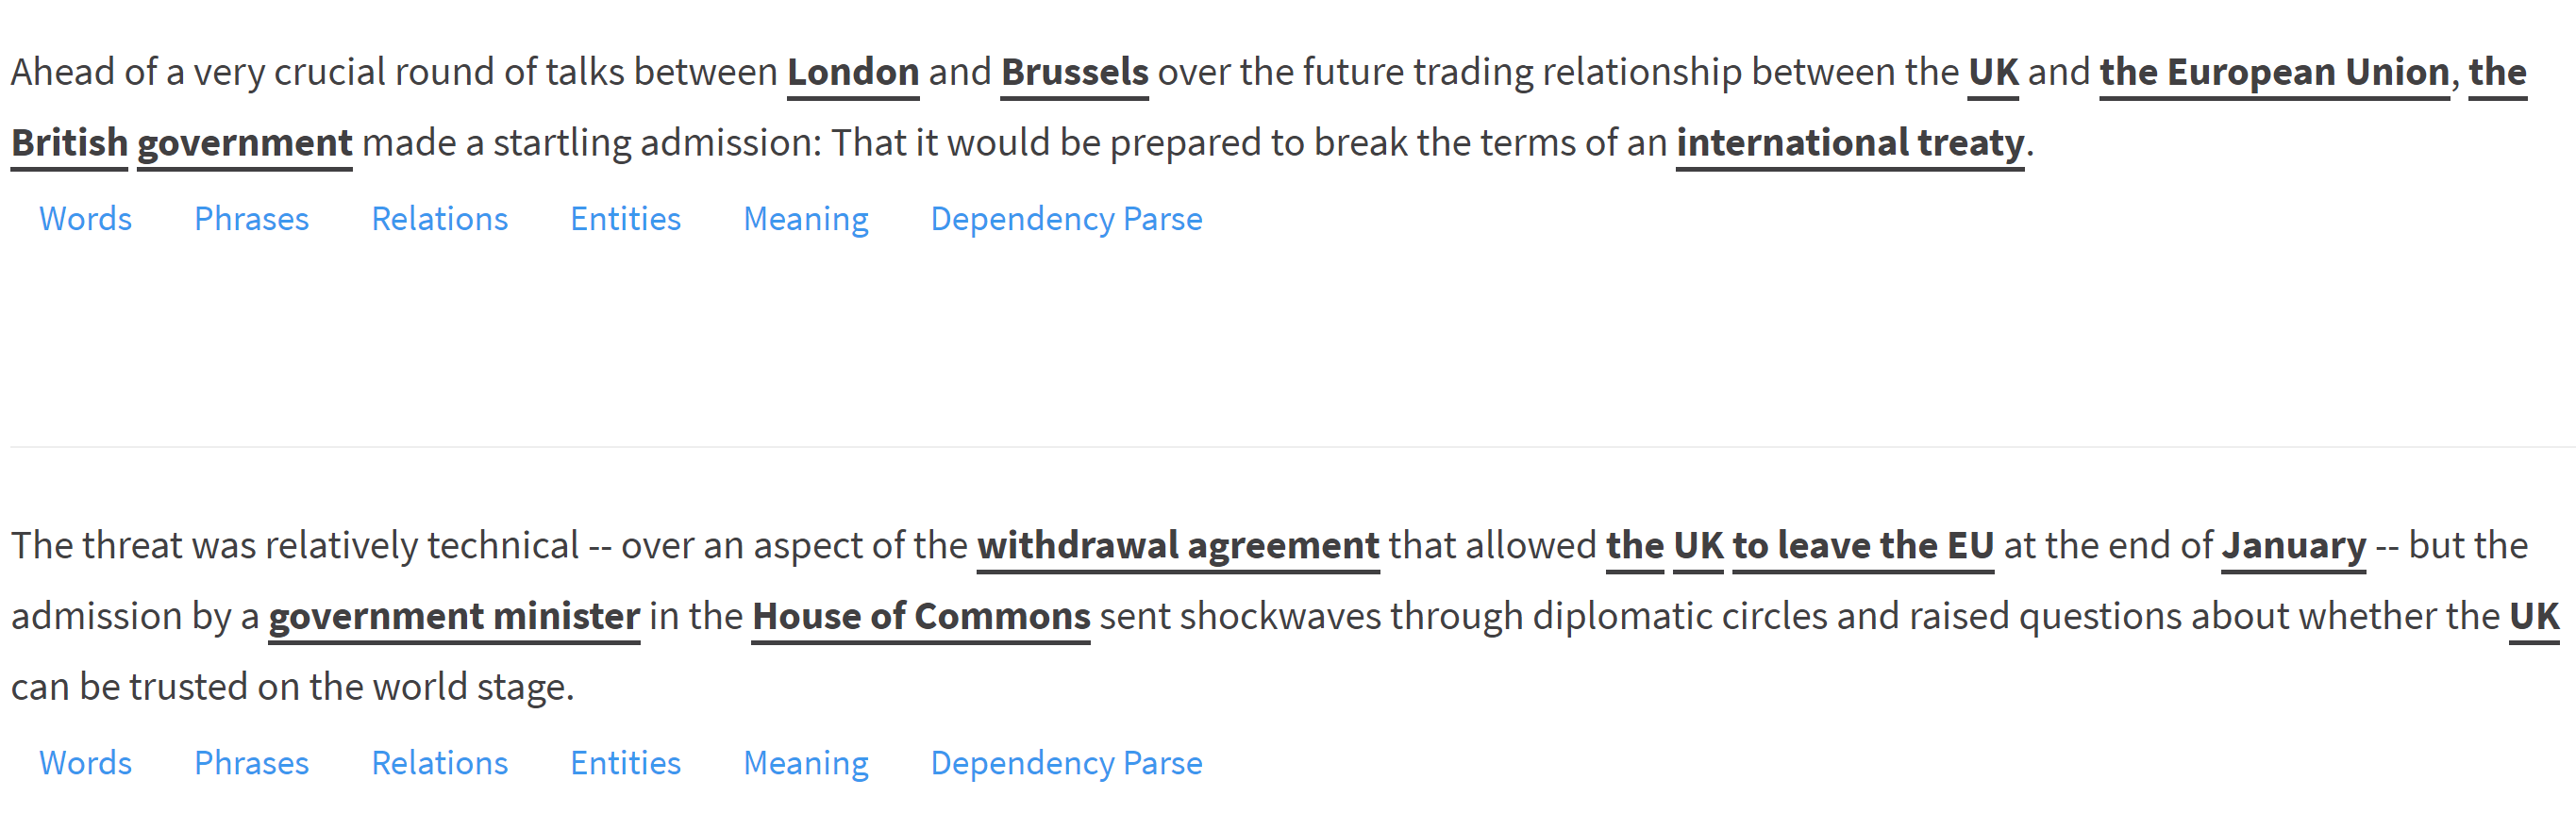
\includegraphics[width=\textwidth]{doc1_textrazor.png}
	\caption{Generated annotations by TextRazor for \citet{mcgee_2020}.}
\end{figure}

We can see that - next to annotating the corpus - TextRazor splits its output per sentence, presumably for sake of readability. Our first observation is that TextRazor has performed  decently in underlining what relevant named entities are. We displayed the results of the performance of TextRazor in table \ref{table:doc1_tr}. We can observe that TextRazor has found all real entities in the sample of \citet{mcgee_2020}, but that it was rather generous in observing entities as well.

\begin{table}[h]
	\centering
	\resizebox{\textwidth}{!}{%
		\begin{tabular}{lllll}
	\textbf{Entity}	& \textbf{Observed entity?} & \textbf{Real entity?} & \textbf{Normalized entity} \\ \hline
		London	& Yes & Yes & London \\
		Brussels	& Yes & Yes & Brussels \\
		UK & Yes & Yes & United Kingdom\\
		the European Union & Yes & Yes & European Union\\
		the British Government & Yes & Yes & Government of the United Kingdom\\
		international treaty & Yes & No & Treaty\\
		Withdrawal agreement & Yes & No & Brexit withdrawal agreement\\
		the UK to leave the EU & Yes & No & Brexit\\
		January & Yes & Yes & 2021-01-01T00:00:00.000+00:00\\
		government minister & Yes & Yes & Minister (government)\\
		House of Commons & Yes & Yes & House of Commons
	\end{tabular}%
	}
\caption{Performance report of TextRazor analyzing the \citet{mcgee_2020} sample.}
\label{table:doc1_tr}
\end{table}

\begin{table}[h!]
	\centering
	\resizebox{\textwidth}{!}{%
		\begin{tabular}{lllll}
			\textbf{Entity}	& \textbf{Observed entity?} & \textbf{Real entity?} & \textbf{Normalized entity} \\ \hline
			150	& Yes & No & 150 \\
			coronavirus vaccines	& Yes & Yes & Coronavirus vaccine \\
			world & No & Yes & N.A.\\
			crisis & No & Yes & N.A.\\
			U.S. & Yes & No & United States\\
			U.S. government & No & Yes & N.A.\\
			Operation Warp Speed & Yes & Yes & Operation Warp Speed\\
			\$10 billion & Yes & No & 10000000000\\
			300 million & Yes & No & 300000000\\
			2021 & Yes & Yes & 2021\\
			The World Health Organization & Yes & Yes & World Health Organization\\
			vaccine & Yes & Yes & Vaccine\\
			eye & Yes & Yes & Eye\\
			two billion & Yes & No & 2000000000\\
			immune system & Yes & Yes & Immune system\\
			infection & Yes & Yes & Infection\\
			health & Yes & Yes & Health
		\end{tabular}%
	}
	\caption{Performance report of TextRazor analyzing the \citet{mckeever_2020} sample.}
	\label{table:doc1_tr}
\end{table}

We can use the results from table \ref{table:doc1_tr} to calculate precision and recall.

precision: 0.7273

recall: 1


\subsection{OpenTapioca}

\begin{table}[h!]
	\centering
	\begin{tabular}{llll}
	\textbf{Corpus}	& \textbf{Model} & \textbf{Precision} & \textbf{Recall} \\ \hline
	\citet{mcgee_2020}	& TextRazor & 0.7273 & 1.0  \\
	\citet{mcgee_2020}	& OpenTapioca &  &   \\
	\citet{mckeever_2020}	& TextRazor &  &   \\
	\citet{mckeever_2020}	& OpenTapioca &  &   \\
	\end{tabular}
	\caption{Test results for TextRazor and OpenTapioca for the corpora}
	\label{tab:doc1_tr}
\end{table}

asdsad

\bibliographystyle{plainnat}
\bibliography{refs.bib}

\end{document}
